\begin{figure}[H]
  \centering
  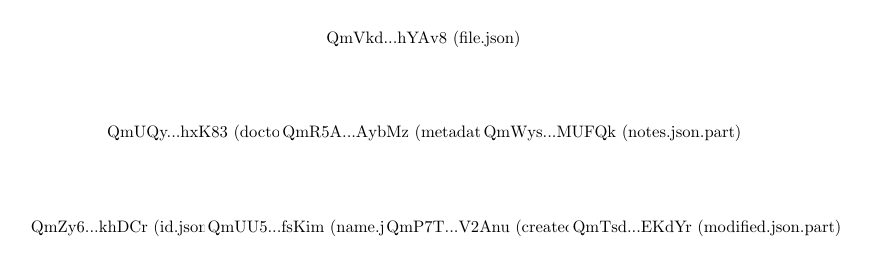
\begin{tikzpicture}[scale = 0.6, every node/.style={scale = 0.6}, every node/.append style={fill = white, rounded corners = 2pt, inner sep = 2pt, align = center}]

  \node at (0, 0) { QmVkd...hYAv8 (file.json) };

  \node at (-4, -2) { QmUQy...hxK83 (doctor.json.part) };
  \node at (0, -2) { QmR5A...AybMz (metadata.json.part) };
  \node at (4, -2) { QmWys...MUFQk (notes.json.part) };

  \node at (-6, -4) { QmZy6...khDCr (id.json.part) };
  \node at (-2, -4) { QmUU5...fsKim (name.json.part) };

  \node at (2, -4) { QmP7T...V2Anu (created.json.part) };
  \node at (6, -4) { QmTsd...EKdYr (modified.json.part) };

  \end{tikzpicture}
  \caption{
    Merkle tree of a JSON file
  }
  \label{fig:json_merkle_tree}
\end{figure}
